%\subsubsection{SVT DAQ}



The SVT DAQ was designed to readout data continuously at 40~MHz from the SVT modules, and transfer data 
to the JLab DAQ once a trigger signal is received. It is based on the same overall architecture as the system 
described in Sec.~\ref{sec:svt_daq}. The largest difference was that with the SVT being only half the size in the 
test run the power and signal aggregation inside the vacuum chamber, as well as the optical conversion part, 
was not needed. This lowered complexity was key to deliver a new working DAQ system in time for the test 
run. The SVT had a total of 20 silicon microstrip sensors, each one connected to an onboard hybrid readout 
card similar to the HPS hybrid, each one holding five 128-channel APV25 integrated circuits, as 
shown in Fig.~\ref{fig:hybrid_and_apv25_testrun}.
 \begin{figure*}[t]
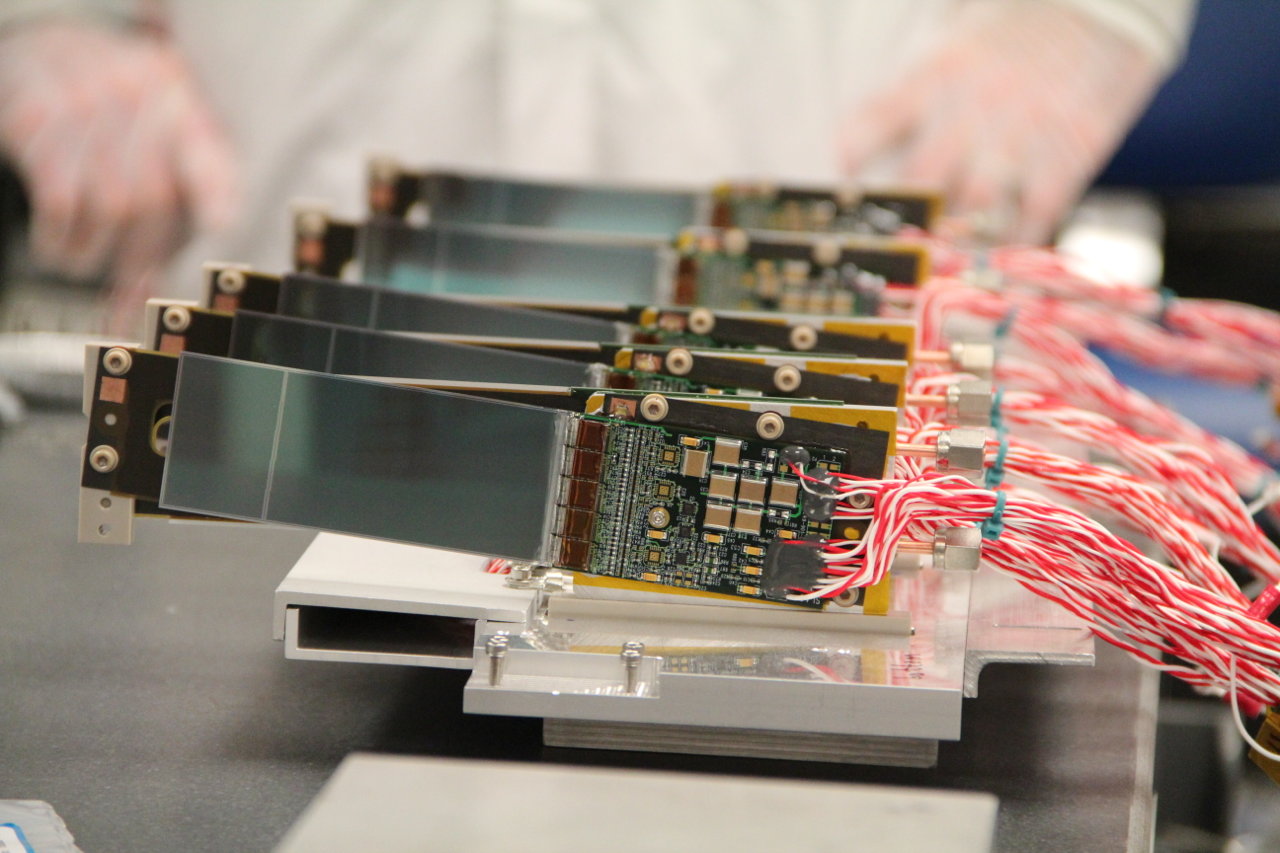
\includegraphics[ scale=0.3]{test2012/daq/svt_modules_on_sup_plate.png}
\caption{\small{View from upstream of one half of the SVT modules mounted on the support plate. Signal, 
power and control are soldered, and potted, to pads at one end while the five APV25 chips are wirebonded 
to the silicon sensor at the other.}}
\label{fig:hybrid_and_apv25_testrun}
\end{figure*}
Contrary to the SVT DAQ for HPS, where front end boards digitize the APV25 analog output signals 
inside the vacuum chamber, the analog signal is carried directly to the ATCA crate located outside the 
vacuum chamber via multi-twisted-pair cable. The amplification and digitization is carried out on the 
Rear Transition Module (RTM) board designed specifically for the HPS test run. 
On the RTM, a pre-amplifier converts the APV25 differential current output to a different voltage output 
scaled to the sensitive range of a 14-bit ADC. The RTM is organized into four sections with each section 
supporting 3 hybrids (15 channels). The ADC is operated at the system clock of 41.667~MHz. 
%The RTM also includes a 4-channel Fiber Optic module and supporting logic which can be used to interface to the JLAB trigger supervisor card.
The ATCA main board, the COB, is similar to the one described for the HPS DAQ 
with the important exception that one of the DPMs functions as the trigger 
interface only and there is no RCE module. Instead, the DPMs package and send the data from the hybrids to 
an external PC through a 1~Gbit/s ethernet connection which serve the same purpose as the 
RCE module in the HPS DAQ. Figure~\ref{fig:svtdaq} shows an overall layout of 
the SVT DAQ system used for the test run (compare to Fig.~\ref{fig:svt_daq_overview}).
 \begin{figure}[t]
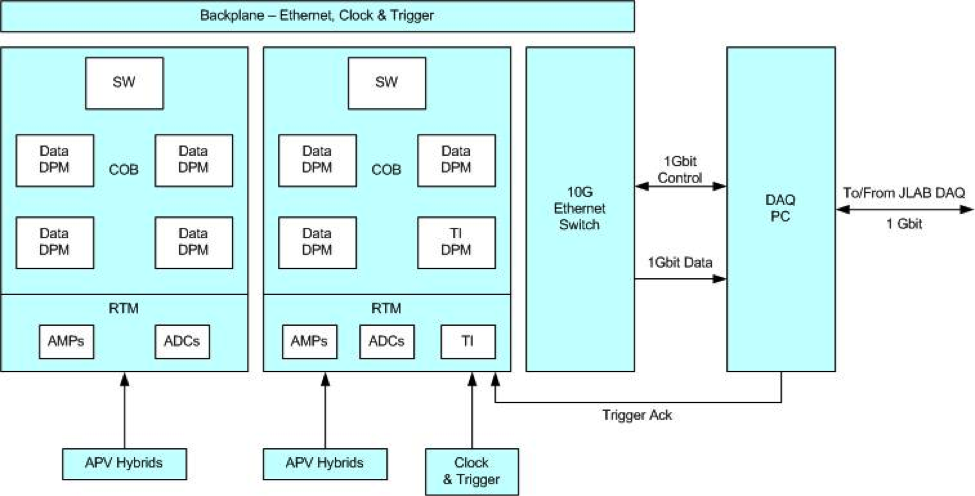
\includegraphics[scale=0.9]{test2012/daq/svt_daq_diagram.png}
\caption{\small{Schematic of the SVT DAQ used for the test run. Note that the hybrids are connected directly 
to the RTM and that an external DAQ PC is used for control and transfer of data to the JLab DAQ.}}
\label{fig:svtdaq}
\end{figure}
The ATCA crate hosts two COB cards, one supporting four data processing DPMs and the other supporting three data processing DPMs and one trigger DPM for a capacity of 21 hybrids, one more than required. 
The test run RTM and COB boards are shown in Fig.~\ref{fig:rtm_testrun}. 
\begin{figure*}[t]
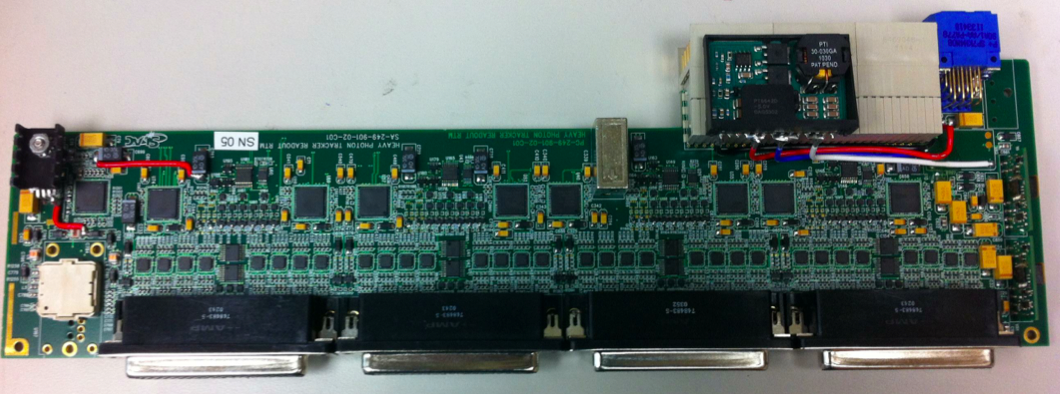
\includegraphics[ scale=0.25]{test2012/daq/rtm.png}
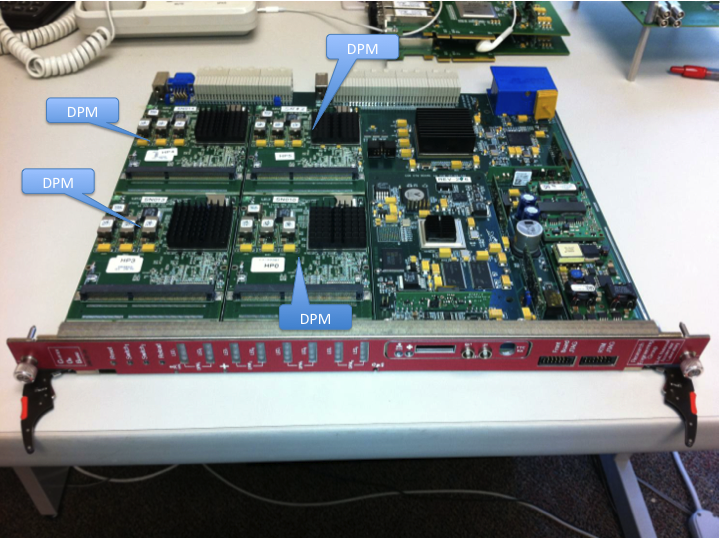
\includegraphics[ scale=0.4]{test2012/daq/svt_daq_module_noted.png}
\caption{\small{Picture of a RTM (top) and COB board (bottom) used in the HPS test run 2012.}}
\label{fig:rtm_testrun}
\end{figure*}
The external PC supports three network interfaces, two standard 1~Gbit/s Ethernet and one custom low latency 
data reception card. The first Ethernet interface is used for slow control and monitoring of the eight 
DPM modules. 
The second Ethernet interface serves as the interface to the JLAB data acquisition system. The third custom 
low latency network interface is used to receive data from the SVT ATCA crate and supports a low latency, 
reliable TTL trigger acknowledge interface to the trigger DPM. This PC hosts the SVT control and monitoring 
software as well as the ROC application described above.
